% \PassOptionsToPackage{prologue,table}{xcolor}
\documentclass[12pt]{article}
%\documentclass[sigconf,anonymous,review]{acmart}


\usepackage{sbc-template}
\usepackage{enumerate}
\usepackage{listings}
\usepackage{xspace}
\usepackage{multirow}
\usepackage{booktabs}
\usepackage{graphicx}
\usepackage{subcaption}
\usepackage{stfloats}
%\usepackage{todonotes}
\usepackage[T1]{fontenc}
\usepackage{etoolbox}
\usepackage[table]{xcolor}
% \usepackage[numbers]{natbib}
\usepackage{hyperref}
\usepackage{wrapfig}
\usepackage{todonotes}
\usepackage{mdframed}

% \lstset{breaklines=true}

% \input{solidity-highlighting}

% \graphicspath{ {./imgs/} }

% \copyrightyear{2024}
% \acmYear{2024}
% \setcopyright{acmlicensed}\acmConference[SBES 2024]{XXXVIII Brazilian Symposium on Software Engineering}{September 30--04, 2024}{Curitiba, Brazil}
% \acmBooktitle{XXXVIII Brazilian Symposium on Software Engineering (SBES 2024), September 25--04, 2024, Curitiba, Brazil}
% \acmDOI{}
% \acmISBN{}

%\setlength\textfloatsep{\baselineskip}


%\newcommand{\scrapper}{https://github.com/PAMunb/mining-email-lists/tree/develop\xspace}
\newcommand{\scrapper}{Removed link\xspace}

% \address{-}
\sloppy

\title{Mining the Questions on Source Code Rejuvenation Asked by C++ Boost Developers}

% \title{Mining Source Code Rejuvenation Questions on C++ Bools Mailing Lists}

\author{anonymous}
\address{-}

% \author{Ismael Medeiros}
% \affiliation{%
%   \institution{Computer Science Department, University of Brasilia}
%   \city{Brasilia}
%   \state{DF}
%   \country{Brazil}
% }
% \author{Fausto Carvalho}
% \affiliation{%
%   \institution{Computer Science Department, University of Brasilia}
%   \city{Brasilia}
%   \state{DF}
%   \country{Brazil}
% }
% \author{Alexandre Ferreira}
% \affiliation{%
%   \institution{Computer Science Department, University of Brasilia}
%   \city{Brasilia}
%   \state{DF}
%   \country{Brazil}
% }
% \author{Rodrigo Bonif\'{a}cio}
% \affiliation{%
%   \institution{Computer Science Department, University of Brasilia}
%   \city{Brasilia}
%   \state{DF}
%   \country{Brazil}
% }

% \author{Fabiano Cavalcanti Fernandes}
% \affiliation{%
%   \institution{Federal Institute of Bras\'{i}lia}
%   \city{Brasilia}
%   \state{DF}\\
%   \country{Brazil}
% }

% \renewcommand{\shortauthors}{Medeiros, I., et al.}

\begin{document}

\maketitle

\begin{abstract}
  Programming languages evolve over time, with new versions being published and new features being introduced, as well as older features being deprecated and discontinued. Existing software that isn't upgraded to use newer versions of its programming language usually contain idioms and workarounds for problems that are already solved, and the process of upgrading to implement these newer versions is called Source Code Rejuvenation. This concept is an important element in software maintenance and development, yet there is still a small amount of research regarding software engineering that focuses on it. This document aims to study how the developers at Boost discussed and dealt with the topic throughout its mailing list history.
\end{abstract}


\section{Introduction}
Programming languages are ubiquitous tools in today's technological development scene. These tools have been present in it for many decades, with the first high-level implementation being created in 1954 - the Fortran language. \cite{howlett1980history} With this historical presence, it is possible to see that popular programming languages evolve over time. \cite{pirkelbauer2010source} This evolution occurs often due to changes in hardware or software constraints or even due to a desire to simplify, modify or extend the use of the tool. As these languages evolve, new solutions are created for problems which had no previously implemented solution. In this sense, the time before the adoption of a new version or modern elements of a language contains many examples of the use of idioms and workarounds \cite{pirkelbauer2010source}, which are solutions to these problems, but applied directly to software written in a language without native support to such a solution. These techniques are often associated with execution problems and code maintenance difficulties. \cite{pirkelbauer2010source}

In an effort to maintain or update a software application, a developer can choose from a number of options to accomplish this task. One of the most common practices is called refactoring, in which changes are made to improve the program's design, while keeping its behavior the same as before. \cite{pirkelbauer2010source} The developer can also choose to adapt the application so that it runs in a more recent version of the original programming language, or use features that are present in the same version but were not previously in use. This type of practice usually adapts code patterns, data structures and other characteristics that are at a lower level of abstraction, transforming them into code at a higher level of abstraction that is more concise and secure. \cite{pirkelbauer2010source} In addition, the adapted code contains information that is better exposed to the programmer and compiler, which would otherwise be very involved in other parts of the code. \cite{pirkelbauer2010source} This practice is called source code rejuvenation.

The C++ programming language is no stranger to such practice. Having existed and being employed for multiple decades, the language has evolved into much more than it originally was. From its original conception of being an extension of C, to its first standardizations in the late 1990's and early 2000's, to its present cycle of 3-year releases, the language has been adapted to needs of various kinds and allowed developers to build even more onto itself as time allowed it and demand incetivized it to. This being the case, the body of code written in early versions of this programming language has no short of examples of idioms and workarounds, especially if those pieces of software are still in use currently. The language's long history of widespread usage and, more recently, increased frequency of new releases, has unavoidably made discussions regarding development and maintenance contain some sort of rejuvenation topics.

Beyond the C++ language itself, there is also the Boost community, who contributed to the language's first and subsequent standardizations. This community consists of voluntary developers who build and maintain C++ libraries that provide extended functionalities to the language. These libraries were important to the creation of the first C++ standard (C++98) and also contributed to the first major release since: C++11. For example, functionalities such as the auto keyword and smart pointers have their origins in Boost libraries\cite{schaling2014boost}. Its contributions to more recent standards have not been as representative as the ones that came before, but they still were helpful for later releases. The community is still active to the present day, developing and maintaining the Boost set of libraries.

Being an entity that has been present since the early times of the C++ language and has had such an important role in its development, this community is bound to have lots of development discussion spanning many years, and consequently many different C++ standards. This is an area of interest regarding source code rejuventaion research, as there may be many things to be learned from how the developers at Boost discussed rejuvenation over its existence.

This document aims to present an effort to apply data mining, natural language processing and thematic analysis techniques to better understand the nature of discussions related to C++ source code rejuvenation, in particular, how it is present in the Boost mailing list. With this effort, it is expected that the results may reveal interesting insights into the overall presence of source code rejuvenation discussions, as well as into the pains that developers face when discussing and/or implementing said changes. These insights would be valuable to incentivize, inform and align further research on the topic and development relating to the rejuvenation issue. This effort also has the added benefit of expanding the known body of collected discussions regarding the source code rejuvenation subject.



%% BACKGROUND AND RELATED WORK ------------------------


\section{Background and Related Work}

\subsection{Source Code Rejuvenation}
Pirkelbauer et al\cite{pirkelbauer2010source} defined source code rejuvenation as a source-to-source transformation that replaces deprecated features with modern code. This concept is related to software engineering as a whole because it names a specific practice that could be confused with others, such as refactoring, in relation to code maintenance and updates. This practice becomes even more relevant as time progresses because, due to the evolution of programming languages, systems that are not regularly updated tend to become outdated, still employing functionalities that have been deprecated or discontinued since their creation. This situation as a whole is more complex than a matter of making higher quality of code or maintaining legacy code, as it is also necessary to take into account the financial aspects and security risks of an update. \cite{sawant2018understanding}

The essence of source code rejuvenation is to detect coding techniques in terms of a lower abstraction level language and convert them to code using a higher abstraction level. Through this process, the code becomes more understandable to programmers and compilers. Unlike refactoring, however, rejuvenation does not necessarily maintain the same behavior of the software in a strict sense, rather, rejuvenation improves it.

An easy-to-understand example of source code rejuvenation, can be seen in how to write the initialization of a data structure containing an arbitrary number of values. Pirkelbauer et al\cite{pirkelbauer2010source} presents the following ways of initializing an object of class \textit{vector} containing types \textit{int} with the values \texttt{[1, 2, 3]} as the usual ways of coding in the C++98 standard:

Option 1: Using consecutive \textit{push\_back} calls

\begin{lstlisting}[language=C++]
vector<int> vec;
vec.push_back(1);
vec.push_back(2);
vec.push_back(3);
\end{lstlisting}

Option 2: Copying from an array

\begin{lstlisting}[language=C++]
int a[] = {1, 2, 3};
vector<int> vec(a,a+sizeof(a)/sizeof(int));
\end{lstlisting}

The author then presents a way of doing the same task with rejuvenated code, using the C++0x standard (currently C++11):

\begin{lstlisting}[language=C++]
vector<int> vec = {1, 2, 3};
\end{lstlisting}

According to the author, the resulting code is more concise, requiring fewer lines of code to perform the same task, and also more uniform, since in this case two different workarounds can be replaced by the same rejuvenated code. This rejuvenation concept is extended to describe many more examples other than the one presented, such as, in the context of C++, \textit{smart pointer} or \textit{lambda expression} usage in place of older constructs and workarounds.

Being our central subject of interest, this concept is taken in at least a general form in this research: the act of porting or adapting existing code from one C++ standard to a newer one. This assumes that the newer version will make use of new features as it may be relevant to that piece of code.

\subsection{Related Work}

The work detailed in this document is similar in nature to other research already done in the field of mailing list/internet forum thread mining and also to other work in the field of source code rejuvenation studies.

Lucas et al\cite{lucas2023embracing} conducted a study on how KDE contributors practice rejuvenation in their projects. The study focused in specific features contained in C++11, C++14 and C++17, and how developers utilized them. The analysis was conducted in 272 KDE programs and libraries written in C++ which projects had started after 2010 and had had at least one commit made in 2022, so as to focus on changes on currently maintained code related to the features contained in post-C++11 versions. The research employed an automated method of detecting increases in use of modern C++ features while the number of actual statements remained constant, in order to determine at what points in time the project could've likely applied a rejuvenation effort. With these results, a keyword search was then applied to further investigate which commit messages were likely to contain rejuvenation efforts, the results of which then were manually analyzed to validate the contents regarding the subject. After this, the authors of the commits that were considered as containing rejuvenation efforts were contacted via email to understand the motivations that led to such a development. The results indicated that the reasoning was often related to improving readability and conciseness of the code, as well as slowing software aging and attracting new contributors to the projects. It's also suggested that the benefits of rejuvenation are perceived by developers, and that programming language designers would benefit from knowing about how modern features are embraced by developers. We referenced this study to set out a general guideline of what to look for regarding the intricacies and importance of source code rejuvenation, not only to the performance and usage of the software in question, but to whoever develops, maintains and manages it. In general, our aim is to understand the main reasons as to why a rejuvenation effort is or is not applied. Additionally, our focus on the Boost community is similar to their sole focus on the KDE community, in our case mainly due to the easily accessible body of data contained in their mailing list and their reputation involving C++ development throughout decades.

Swillus et al\cite{swillus2023sentiment} conducted an analysis of Stack Overflow posts regarding software testing. While also focusing on a widely applied and influential topic on software development, the analysis focused on how this practice is perceived through the developer's perspective. For this, the Stack Overflow messages were mined and subsqeuently filtered through a semi-automated method and then by a systematic qualitative data analysis. These processes intend to both find posts relevant to the topic and to initiate the construction of preliminary hypotheses for further analysis. The strategy employed for the manual data analysis was based on the Socio-Technical Grounded Theory\cite{hoda2021socio}, and required iterative cycles envolving teams of analyzers in order to achieve its goal of determining and characterizing the interpretative contents in the body of data. Added to this, an automated sentiment analysis was employed to verify the sentimental response each topic of interest had. Their results suggest that software testing motivation increased with the complexity of the project, and that the practice itself is seen as something to aspire to. We referenced this research in order to employ a somewhat similar manual analysis method focusing on broader interpretative topics.

Tahir et al\cite{tahir2020large} conducted a similar style of research investigating how developers at Stack Overflow, Stack Exchange and Code Review discussed code smells and anti-patterns. The authors employed similar automated filtering techniques, given the similarities of the platforms in question, and subsequently employed a manual effort on validating the automated results and further analysing the thematic contents of the dataset. Their results suggest that developers don't have a clear definition of code smells and anti-patterns, yet they seem to have negative feelings towards these practices in general. Similarly to the previous research mentioned, we also referenced their work for employing a similar thematic-focused approach.

Throughout the studies mentioned, a common theme is that of data mining in order to obtain a dataset to apply the analysis upon. These and many other published studies of similar application were the main source of inspiration to proceed this way, having a clear idea of what the Boost mailing list might contain given its large span of messages over decades. Our study is not meant to be an extensive, final search for source code rejuvenation in the Boost mailing list. Instead, we aim to find as much general rejuvenation discussion as possible and analyze how it was handled, as well as maintaining references to these messages, should any interested person wish to use it.


\subsection{Natural Language Processing and Learning Algorithms}
Natural language processing (commonly abbreviated to NLP) is an area of research that explores how computers can be used to understand and manipulate natural language in text or speech. it is an endeavour that aims to gain knowledge about how humans understand and use language, as well as to develop tools and techniques that allow a computer to perform tasks that involve manipulating and understanding natural language. \cite{chowdhary2020natural}

\subsubsection{Data Vectorization}

In order to employ a machine-learning algorithm to classify messages regarding their relevance to source code rejuvenation discussion, there needs to be a way to process the text using metrics and organize it in a way that the learning algorithm can receive as input. The NLP approach chosen for this task was a technique called Bag of Words, which is responsible for extracting the features of the input text. In it, three main processes are employed:

    \begin{itemize}
    \item{\textbf{\textit{Tokenization}}}
    
    The process that divides all text strings into pieces called tokens. It uses, for example, spaces and punctuation as separators. Each unique token is identified by an integer.
    
    \item{\textbf{\textit{Counting}}}
    
    The number of occurences of each token in the input data is counted and stored.
    
    \item{\textbf{\textit{Normalization}}}
    
    The distribution of tokens is normalized, with weights applied to each token, seeking to reduce the importance of those that appear in a majority of the inputs.
    
    \end{itemize}

With this technique, it is possible to extract the irreductible elements of meaning (words) present in different texts, and check how often each element appears.

It is also worth mentioning that the process of normalization mentioned above can be done using the TF-IDF transform. This transform multiplies the frequency that a given term occurs in an input (term-frequency, or TF) by its inverse frequency of occurence in different inputs (inverse document-frequency, or IDF). Thus, if a term is used very frequently and in many documents, such as words that carry little individual information, like articles, prepositions and the like, this term will not be of great significance in the extraction result, even if it is very common within the body of data.

Using the TF-IDF transform makes it easier to filter out tokens that would not be as relevant in terms of meaning in order to better characterize each message or input.

The features obtained through this technique can then be used to create a machine learning model that is a message classifier. This classifier should be able to identify messages that are or are not relevant in relation to the topic of source code rejuvenation. For this task, a learning algorithm called Support Vector Machine was used.

\subsubsection{Support Vector Machines}
Commonly abbreviated as SVM, Support Vector Machines are a family of learning algorithms that specialize in two-class discriminant functions. \cite{mammone2009support} The case of classifying text messages with regard to topic relevance is about establishing a threshold that separates relevant messages from non-relevant ones, and this is precisely the task an SVM performs.

In short, the goal of an SVM algorithm is to efficiently search for a separating hyperplane in a high-dimensional space of features. \cite{mammone2009support} In other words, given a feature space generated by metrics and other heuristics applied to the body of data, the SVM searches for a linear threshold that separates the data entries into two classes according to the given specifications. This threshold is called a hyperplane, due to it being its representation in high-dimensional space. In the application described in this document, the separating hyperplane's function was adjusted using the Stochastic Gradient Descent Technique.

The algorithm, in its simplest form, aims to find the hyperplane that separates the two data sets perfectly and that maximizes the margin between the hyperplane and the data points closest to it. This model is called the maximum margin classifier, or strict margin SVM. \cite{mammone2009support}

Since real-world applications rarely have data sets that are perfectly or even linearly separable into categories, there are extensions to this original algorithm. In order for the algorithm to accept miscalssifications up to a specified margin of error, so that is can be applied to datasets with more noise and outliers, there exists the soft margin classifier. In addition, so that the algorithm can deal with data sets that are not linearly separable, Kernels (or kernel functions) are used to manipulate the feature space consistently, so that the threshold can be computed linearly. \cite{mammone2009support}


\section{Study Settings}

The goal of this research is to understand {\color{red} REVISAR}
as reflected in the questions and answers on the Boost mailing lists.
Boost is one of the main C++ open-source organizations, significantly contributing to the evolution of the C++
language specification. Currently, hundreds of C++ developers contribute to the implementation of Boost libraries,
which are widely used and often integrated into the C++ standard library. Indeed,
the success of some Boost libraries can be partially attributed to a formal review
process that relies on mailing list discussions. Considering that the Boost foundation contributes to the evolution
of C++ standards, it is expected that Boost libraries would be up-to-date with new versions of the language.
However, migrating a Boost library to a new version of the C++ programming language is anything but trivial and
should be carefully discussed among Boost members (Figure~\ref{fig:email1} shows a snippet of an email thread from the
Boost mailing list on this subject). These careful discussions are necessary because rejuvenating a library
might not only lead to (unexpected) breaking changes but also require the clients of that library to update their C++ code, dependencies,
compilers, and tools as well. 

\begin{figure}[htb]
\begin{mdframed}[backgroundcolor=gray!40,shadow=true,roundcorner=8pt]
  \begin{small}
> Pursuant of discussion elsewhere: \\
> Does anyone have any concrete objections to Boost moving to \\
> a C++14 baseline? \\

Yes. I do.(Caveat: But I'll be happy to be over-ruled.)

We recently established that C++/Boost are unique in so far as they provide high-level abstractionson top of the C++ language. This C++ language creates optimized, compiled object that is near enough to the machine to facilitate high-performance. Along those lines, a lot of clients use Boost/C++ with older compilers, not because they cherisholder compilers, but since constraints make them end up stuck there. These are constraints such as legacy customer projects, old compilers, legacy licenses, [...], and more. Boost provides a service.
\end{small}
\end{mdframed}
\caption{Example of an email thread highlighting the challenges of rejuvenating Boost libraries due
  to compatibility issues with client programs, compilers, and so on.}
\label{fig:email1}
\end{figure}

\subsection{Research Questions}

To understan {\color{red}REVISAR}, we investigate the following research questions:

\begin{enumerate}[(RQ1)]
  \item How prevalent are code rejuvenation discussions in Boost mailing lists?
  \item What are the most common themes in code rejuvenation threads?
  \item What topics are most frequently discussed in these threads?
  \item Which C++ language standards are mentioned most often?
\end{enumerate}


Answering the first research question allows us to measure the extent of code rejuvenation present in the entire mailing list history. Estimating how frequently software developers at Boost discuss this topic can help gauge its prevalence and importance to them.
Answering the second research question enables a deeper dive into the content of these discussions. It is crucial to understand the themes that emerge, particularly to justify positions taken regarding code rejuvenation. We aim to identify the most commonly used arguments by both proponents and opponents of rejuvenation, providing insights into the reasoning and priorities of each developer involved in the discussion. Finally, answering research questions RQ3 and RQ4 helps us understand the specific topics addressed in messages about code rejuvenation. Given the nature of rejuvenation, it is of interest to identify which C++ standards were most frequently discussed.

\subsection{Data Collection}

% %% STUDY PROCEDURES ----------------------------------

% \section{Study Procedures}

% The research effort was initiated with the collection of data for the study. For that, the development of a web scraping application was conducted. This application scraped and stored the contents of the \textit{Boost mailing list}\footnote{https://lists.boost.org/Archives/boost/} into a database application. The details of this application are found in section 4.1.

% Following the collection of data for the study, a manual effort was conducted to collect a body of known messages that were deemed as relevant to the topic of source code rejuvenation. This body is a subset of the whole mailing list and was used in order to employ a machine learning application to reduce the scope of the research.

% Since it was expected that the relevant amount of messages within the whole mailing list would be a very small portion of it, a classifier model was created in order to analyze the whole mailing list in an automated way, and give preliminary insight into which messages were relevant or not. The manually selected body of relevant messages, along with messages known to be relevant from previous research efforts and also randomly sampled messages from the mailing list were used as both training and test databases for the classifier model. The details of this implementation are found in section 4.2.

% Having employed the classifier model, the messages it deemed as relevant were then manually reviewed in order to both filter out false positives and to establish potentially relevant threads for further analysis. In this case, both the message itself, as well as the thread it belonged to were analyzed, considering if the thread could potentially contain more discussion on the topic of source code rejuvenation that was not identified by the classifier model. These threads were then read in full, in search of relevant messages. These messages, as they were selected, were also analyzed manually regarding their bias towards rejuvenation, their main arguments and what C++ standards were referenced. The details of this effort are found in section 4.3.

% \subsection{Web scraping and the resulting database}

% % Starting off the study, there was a need for a body of data to be studied.


Our focus is on the Boost community, and the most readily available data for our research is contained in their public message board: the \textit{Boost MailMan Archive} (referred to hereafter as the \textit{Boost mailing list}). This archive is a message board hosted on a static HTML website, making it easy to collect data using a web scraper. We built a scraping application that goes through every post in the mailing list and captures key information such as the date of posting, author name, title of the post, and the body of the message. The scraper stores the collected data in a relational database for later access. In March 2023, we collected all the data available on the Boost mailing list at the time: a total of 253,548 messages, spanning more than two decades of mailing list history (from February 1998 to March 2023).

% \subsection{Message Classifier}

To better handle the volume of data collected, we decided to employ an automated
effort to reduce the scope of our manual data analysis procedures. For that,
our decision was to explore the Support Vector Machine (SVM)~\cite{\cite{mammone2009support}} algorithm to classify the messages
that were more likely to contain code rejuvenation discussion.
  
SVM requires a labeled dataset for both training and testing of the model. As such, we
employed a manual search effort in order to find a small amount of messages we deemed relevant to the topic.
In it we went through many different points in the mailing list's history and searched through the threads
for possible rejuvenation discussion. Once we found a relevant message, we stored its URL and relevant information
in a spreadsheet for future reference. Adding messages known from previous research efforts,
we found 58 messages in this endeavor, of which 32 were used to train the model and the remaining 26 were used for testing.

\todo[inline]{n\~{a}o consegui compreender muito os numeros no paragrafo anterior e no proximo paragrafo.}

The training dataset was composed of 32 manually selected messages and 300 randomly selected messages from the mailing list. The manually selected messages were
labeled as ``relevant to rejuvenation'' and the 300 randomly selected were labeled ``not relevant to rejuvenation''. Similarly, the testing
dataset was composed of 26 manually selected messages and 20 randomly selected from the mailing list. They were labeled the same
way as the training dataset.

The classifier model first performs the vectorization of the training dataset, using a TF-IDF transformation
to more accurately represent relevant tokens in the analysis. Afterwards, the vectorized data is given as input
to the learning algorithm. This results in a classifier model that we can leverage to classify new messages.
To test the resulting model, the testing dataset is vectorized in the same way the traning dataset was, then we use the
model to classify this new dataset's entries. Since this dataset was previously classified,
we can measure the model's performance with metrics such as precision and recall.

We obtained a score of 71\% precision and 100\% recall for ``not relevant to rejuvenation'' messages. We also got 100\% precision and 69\% recall for ``relevant to
rejuvenation'' messages. Our objective here was to automatically find more messages ``relevant to rejuvenation'' than what we already had in our notes and spreadsheets.
For that, 69\% recall in a small corpus of 46 test messages was likely to return many more true positives when applied to the full dataset of
250 thousand messages. Therefore, we considered this model acceptable to search for more rejuvenation-related messages. This also means, however,
that this approach will not be an extensive search, due to the low amount recalled.

Running the whole mailing list dataset through the classifier model returned 967 messages labeled as ``relevant to rejuvenation''. Not every single one of these was
manually reviewed, as will be explained in the next section. However, of the ones manually reviewed, 37.4\% (161 messages) were considered
relevant to code rejuvenation.

\todo[inline]{Discutir o par\'{a}grafo anterior}
\subsection{Manual Analysis Effort}

\todo[inline]{Incluir percentuais nos n\'{u}meros abaixo}

Having the results from the classifier, we employed a manual effort in order to open the scope of analysis further out than only the model's results. For this, we went through the messages obtained from the automated effort and analyzed all threads to which they belonged to. By analyzing both the contents of these messages and the overall scope of discussion present in the thread as a whole, we considered if the threads were likely to contain a substantial amount rejuvenation-related discussion, also considering the model's results as an indication, such as when the model labeled tens of messages from a single thread as rejuvenation-relevant. If that was the case, we selected those threads for further analysis. Since many messages in the model's results belonged to reocurring threads, not every message from the results needed to be read then, as they would be later when the thread itself was read through. After this process, we selected 62 threads marked as ``potentially containing rejuvenation-related messages'', which opened the scope to 2816 messages in the threads.

We then manually went through every message in this corpus of message threads. At this point, having already read through many instances of rejuvenation-related messages, we derived a rough list of reocurring categories of arguments present in rejuvenation-related discussion. This list would be updated as we read through the messages in the selected threads.

In this manual classification process, we first consider if the message in question contains rejuvenation-related discussion. To determine that, we consider if the message contains any arguments for rejuvenating, against a previously proposed rejuvenation effort or related to rejuvenation, but ambiguous or neutral towards it. If it had at least one of these, it would be considered as containing rejuvenation discussion and would be added to a spreadsheet. The results of this would be used to answer our first research question.

As a message was selected for containing rejuvenation-related discussion, it also was classified in three ways. Firstly, we consider \textbf{rejuvenation bias for the whole message}. That is, if the message as a whole can be said to be arguing for rejuvenation, against rejuvenation, is not clearly defined, or is neutral towards it. Afterwards, seeking to categorize the contents of the message in more detail, we consider \textbf{what topics were discussed} in that message. We considered mainly C++ standards (from 98 to 20) as topics, but there were also topics labeled as ``General'' and ``Compilers''. If a message mentioned any of these topics, it would be marked as having discussed it. Last but not least, we consider \textbf{what arguments were proposed} in that message, and note them down in the spreadsheet. For this, we tried to categorize the most reocurring arguments in these discussions into a list, as mentioned previously. Whenever we encountered an argument point in a message, we could reference that list to categorize it as one of the categories we already had, or create new categories not previously included.

Going through every one of these message threads, we determined that two of them were not related to rejuvenation, rather, were related to an adjacent, but otherwise not related topic: Backporting code. These threads were excluded from the body of analysis, resulting in a body of 60 threads, containing 2639 messages. After every message was read, analyzed, selected and classified if selected, we obtained a body of 603 messages considered as containing rejuvenation-related discussion. Every single one of these messages had at least one topic and one argument related to it, and had been classified according to rejuvenation bias.

% ANALYSIS RESULTS ------------------------------




\section{Analysis Results}
The analysis was guided by the previously mentioned research questions. This section will then be organized to answer them in order.

\subsection{Prevalence}

To answer research question (1) in the most broad sense possible, it is necessary to look at how many messages we found that discuss rejuvenation.

The total number of messages collected from the mailing list was 253,548. Also, from the research procedures, we found 603 that were considered as containing code rejuvenation discussion. With this, those 603 messages represent 0.24\% of the total amount. Since this was not an extensive search for those messages, we will consider this, at most, a lower bound.

{\color{red}If we were to trust blindly the selection of threads that was conducted before the manual analysis, assuming every message in every thread selected contained rejuvenation-related discussion, that would be a total of 2639 rejuvenation messages. This represents 1.04\% of the total amount, which we will consider a naive upper bound.

\textbf{Therefore, a rough estimate for how much of the total messages were related to code rejuvenation is between 0.24\% and 1.04\%.}}

Analyzing further, of the 603 selected messages we found the distribution of occurrences present in Figure \ref{fig:msg_year}. Figure \ref{fig:prop_year} indicates what percentage those message occurrences represented of the total number of messages posted in that year. Of those distributions we get an average of 23.2 rejuvenation messages per year and 0.48\% presence per year.

From the manual analysis we determined that the discussions before and after 2011 were fundamentally different in nature. Before 2011 rejuvenation discussion was basically only about compiler support. With the release of C++11, the messages from 2011 onwards are much more like what we expected of code rejuvenation discussion, talking mostly about language standards and features and why to use them or not. This type of discussion relates more to language evolution, as opposed to the compilers available. Not to mention, rejuvenation discussion was much more frequent from 2011 onwards, as is evident in the distributions shown.

Analyzing the same data but limiting the scope to only 2011 onwards, we get an average of 43.2 messages per year, and an average of 0.94\% presence per year.

Moreover, from 2011 onwards the total number of messages collected is 80,043, which is significantly smaller than the whole corpus of messages. However, considering the estimates calculated previously, the number of messages selected manually drops only to 562, which gives us a lower bound of 0.7\% of presence.

\begin{figure}[h]
  \centering
  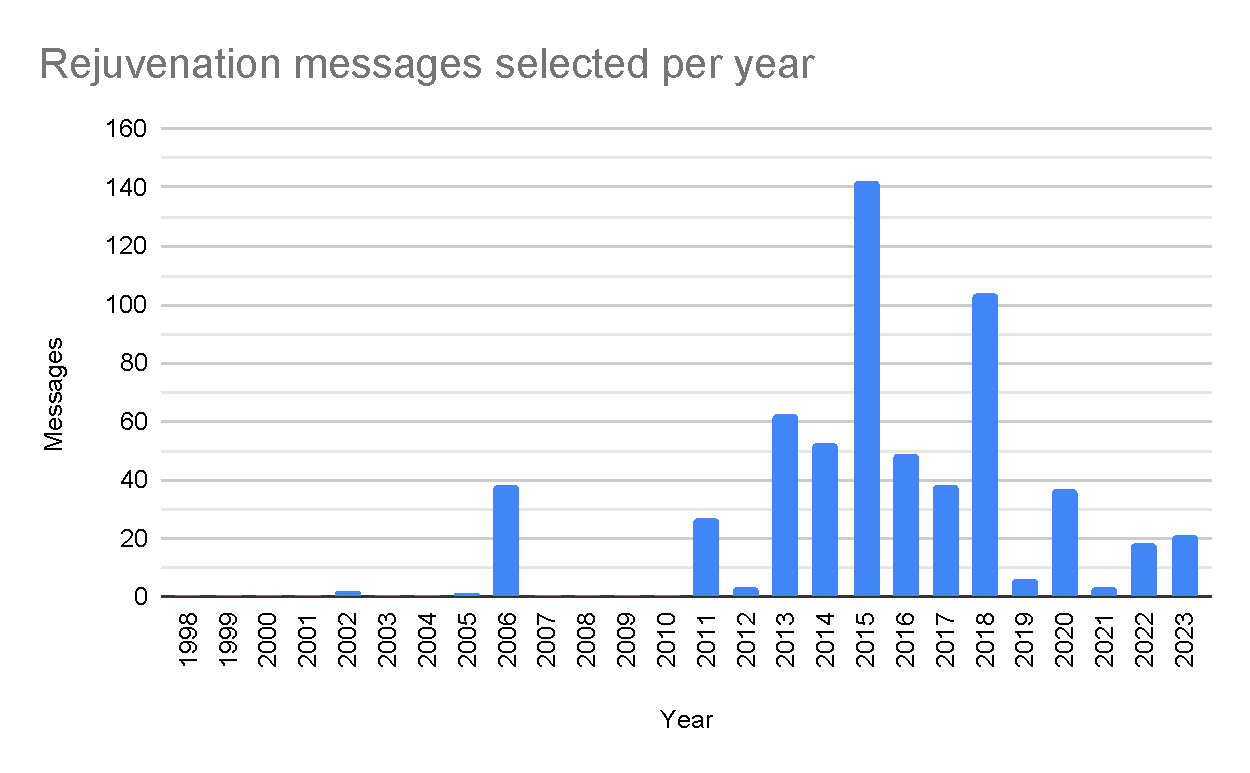
\includegraphics[width=\linewidth]{images/rejuv_msg_per_year.pdf}
  \caption{Distribution of rejuvenation messages found by year}
  %\Description{A histogram of how many messages related to source code rejuvenation were found in a given year from 1998 to 2023 in the Boost mailing list.}
  \label{fig:msg_year}
\end{figure}

\begin{figure}[h]
  \centering
  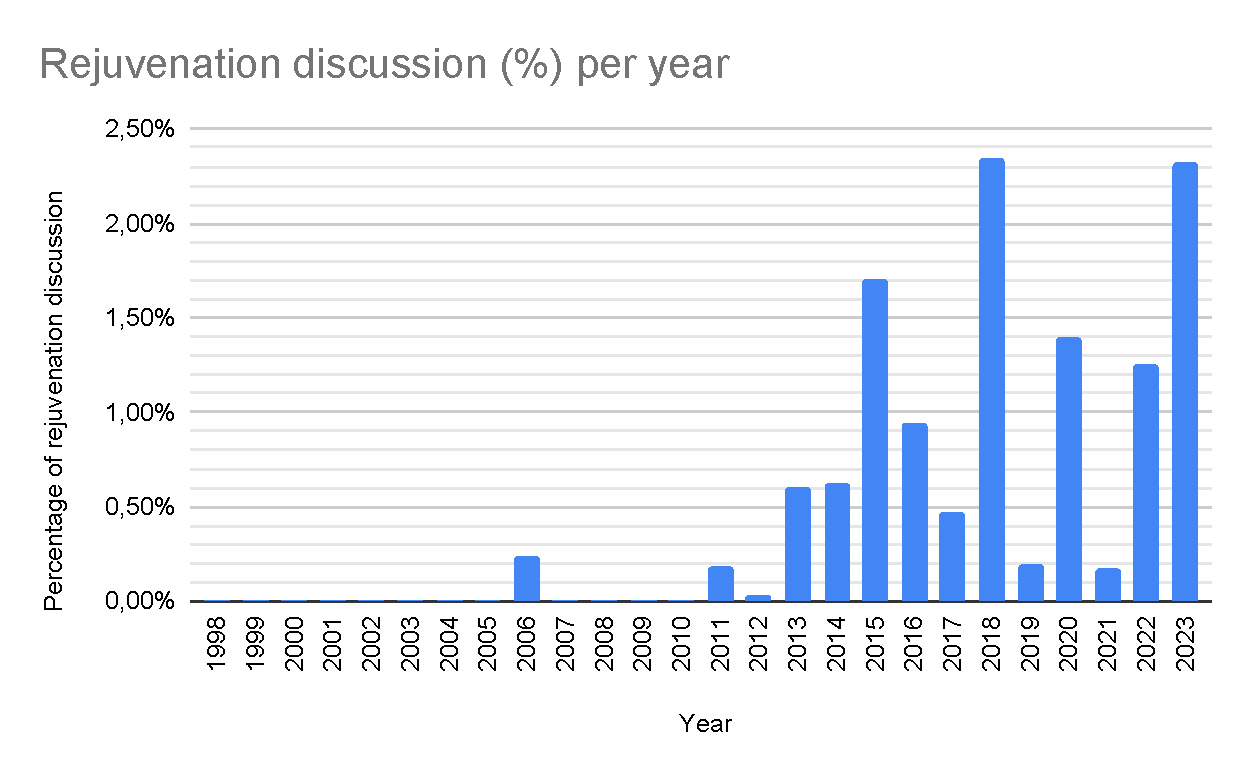
\includegraphics[width=\linewidth]{images/rejuv_proportion_per_year.pdf}
  \caption{Percentage of rejuvenation messages found by year}
  %\Description{A histogram of how much of the messages were related to rejuvenation from the total messages posted in a given year from 1998 to 2023 in the Boost mailing list.}
  \label{fig:prop_year}
\end{figure}

{\color{red}The naive upper bound is affected similarly. From 2011 onwards, the number of messages contained in the selected threads is 2532, which now represents 3.16\% of the total amount.

\textbf{Therefore, a rough estimate of code rejuvenation discussion presence from 2011 onwards is in between 0.7\% and 3.16\%.}}

These message distributions, however, pose a contradicting trend. Even though total code rejuvenation-related message numbers declined after 2018, the percentage those numbers represent from the year's total messages have an increasing trend. This can be explained by an overall trend of reduced usage of the Boost mailing list, which was attributed in some messages inside the mailing list to developers moving discussions to GitHub, Slack, and other platforms. This fact also explains the dramatic reduction in the total number of messages collected on the analysis from 2011 onwards.

What this suggests is that \textbf{source code rejuvenation discussion increased in presence even though the mailing list saw decrease in usage.}

Furthermore, analyzing the distribution of messages per year in relation to what was the most recent C++ standard in each year yields an interesting result. In Figures \ref{fig:std_msg_year} and \ref{fig:std_prop_year} we can clearly see peaks in 2015 and 2018. The red color representing C++14 as the most recent standard released and the green color representing C++17, those two peaks seem to align with C++ releases with a 1 year delay. This does not happen equally for C++11 (yellow) nor C++20 (blue) however, although there are peaks in their respective sections.

\begin{figure}[h]
  \centering
  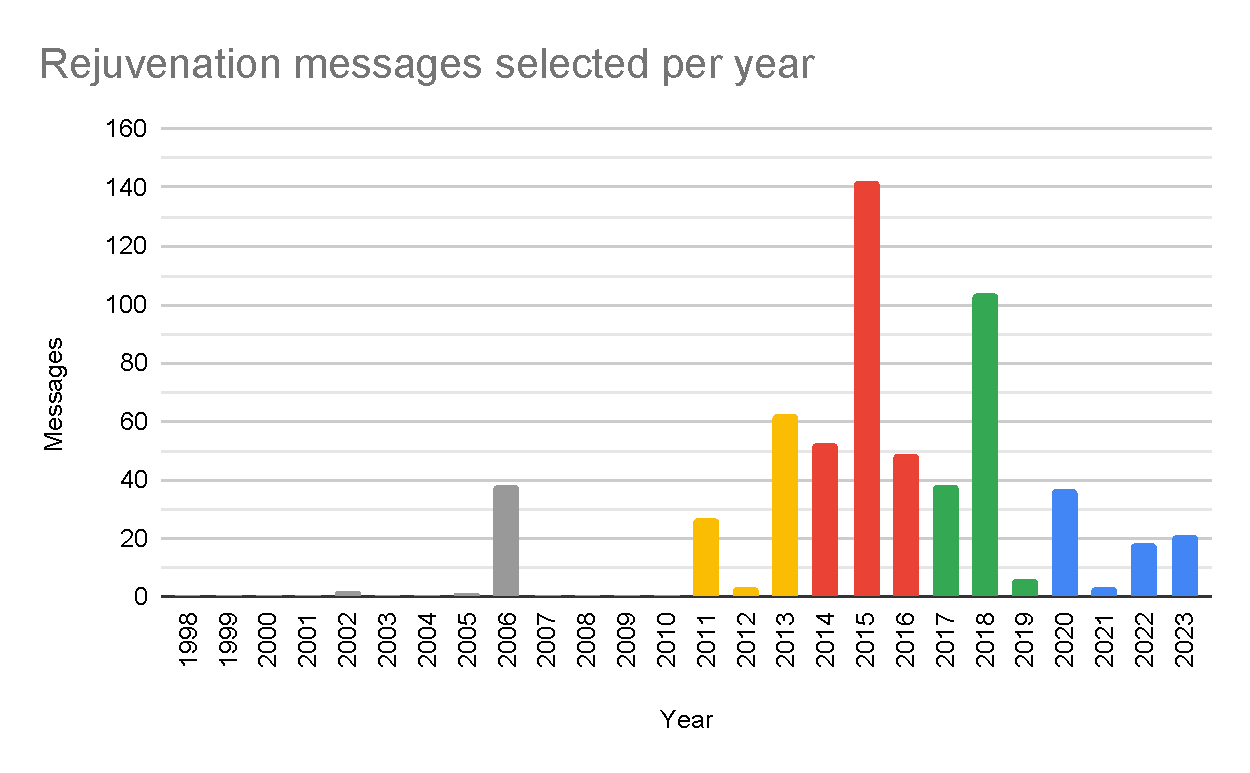
\includegraphics[width=\linewidth]{images/rejuv_msg_per_year_std.pdf}
  \caption{Distribution of rejuvenation messages found by year, colored by most recent C++ standard}
  %\Description{A histogram of how many messages related to source code rejuvenation were found in a given year from 1998 to 2023 in the Boost mailing list. The bars are colored according to what C++ standard was the most recent one available at that year.}
  \label{fig:std_msg_year}
\end{figure}

\begin{figure}[h]
  \centering
  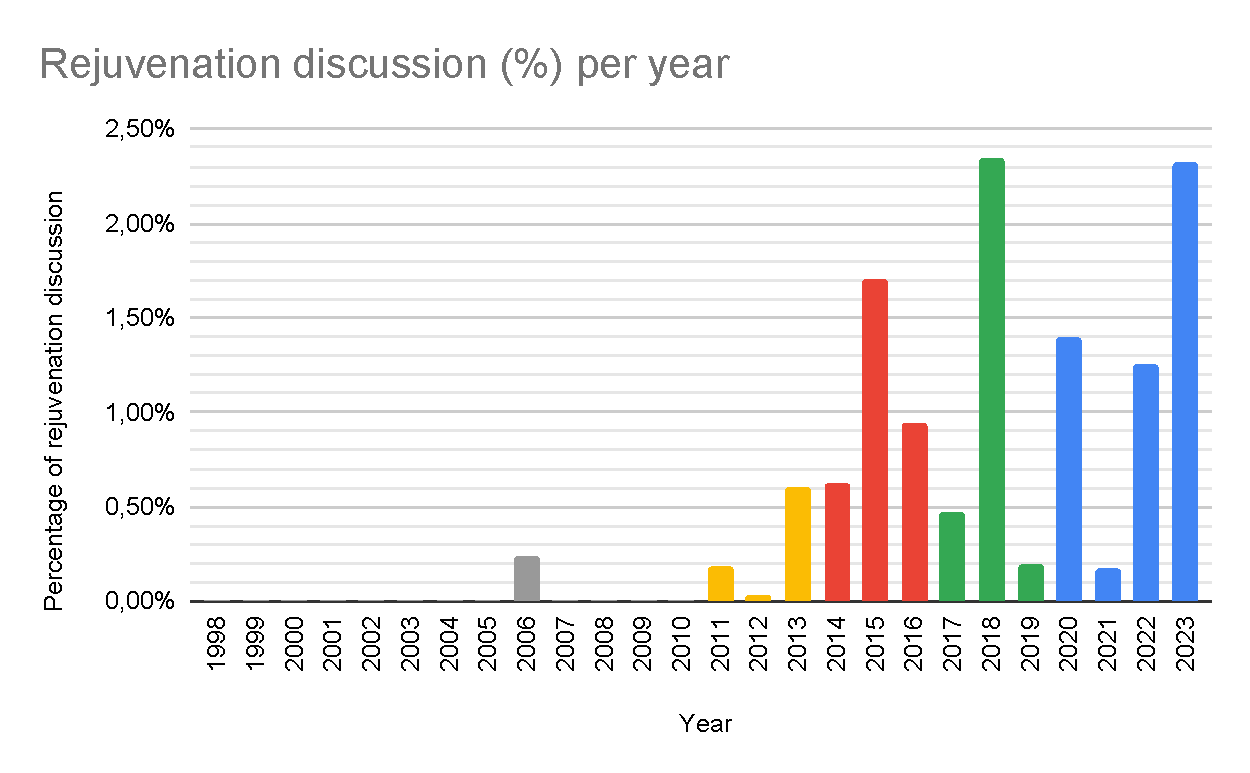
\includegraphics[width=\linewidth]{images/rejuv_proportion_per_year_std.pdf}
  \caption{Percentage of rejuvenation messages found by year, colored by most recent C++ standard}
  %\Description{A histogram of how much of the messages were related to rejuvenation from the total messages posted in a given year from 1998 to 2023 in the Boost mailing list. The bars are colored according to what C++ standard was the most recent one available at that year.}
  \label{fig:std_prop_year}
\end{figure}

\textbf{This suggests a correlation between code rejuvenation discussion occurrence and C++ standard releases.} The 1-year delay observed can be explained due to resistance in adhering to new standards as soon as they're released, either due to bugs in the standard or low expected adherence from C++ developers.




\subsection{Topics}

To answer research question (2), a list of topics was derived, as mentioned previously. For every message selected as rejuvenation-relevant, we noted down what topics were mentioned in it. Within the 603 messages analyzed, there were 998 occurrences of topics, which gives an average of 1.7 topics per message. \textbf{This suggests that messages often talked about more than one topic.}

Of the topics themselves, the occurrence distribution is found in Figure \ref{fig:topic_occurr}. \textbf{The two most mentioned topics were C++11 (mentioned in 50.9\% of messages) and C++03 (40.3\%).} This dominance, paired with the knowledge that the vast majority of these analyzed messages occurred after 2013 (as visible in Figure \ref{fig:msg_year}), suggests that \textbf{there were many discussions regarding these C++ standards many years after their releases, while more recent standards were not discussed as much.} In the case of C++03, in most of its occurrences, it had already completed a decade after its release. C++11 also was mentioned a fair amount 5+ years after its release.

\begin{figure}[h]
  \centering
  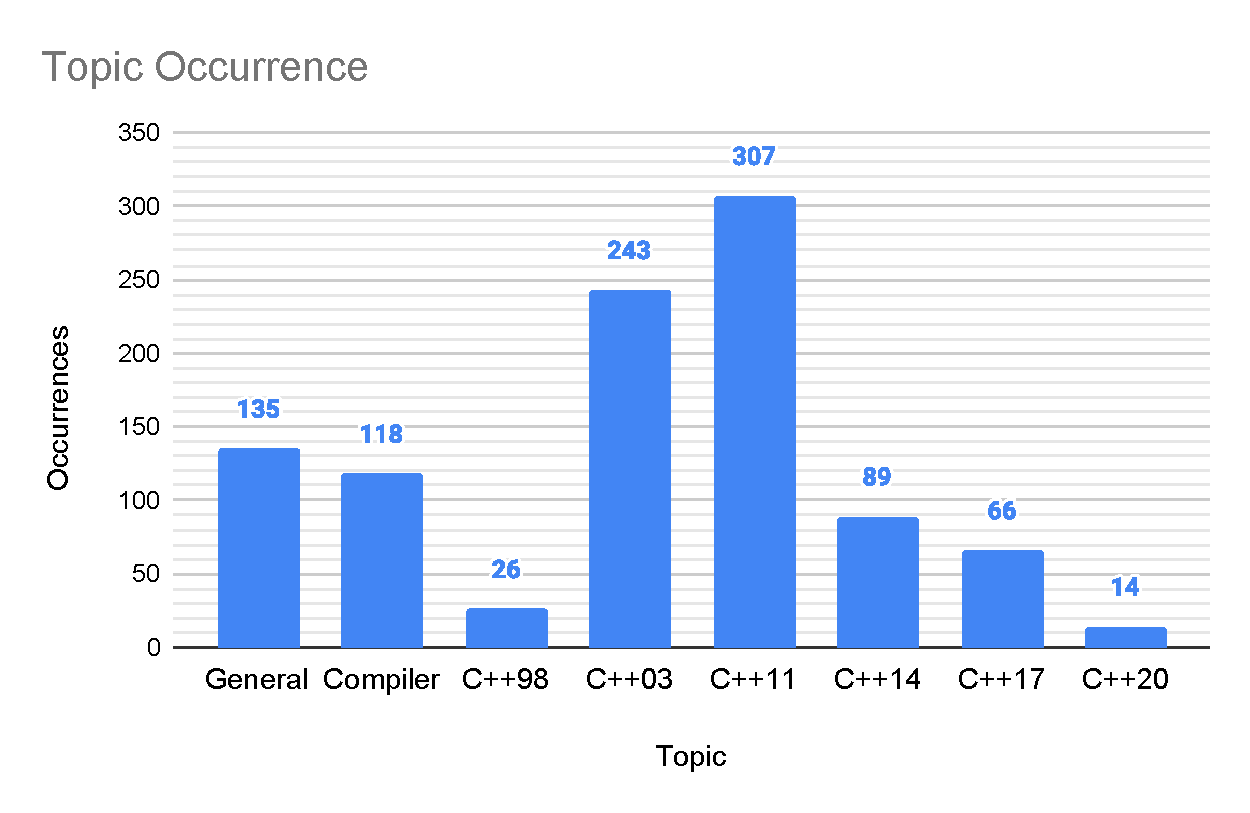
\includegraphics[width=\linewidth]{images/topic_occurrence.pdf}
  \caption{Bar graph of occurrences of topics within rejuvenation discussion}
  %\Description{A comparison between the topics listed and tracked, showing how many times each one occurred in the dataset.}
  \label{fig:topic_occurr}
\end{figure}

While analyzing the distribution of each topic by year, we noticed, as shown in Figure \ref{fig:cpp03_11_year}, that, besides being the most popular topics overall, the occurrences of C++03 and C++11 seemed to correlate heavily with one another. In the joint histogram, it is possible to see many similar peaks between the two topics, most notably in 2011, 2015 and 2018.

\begin{figure}[h]
  \centering
  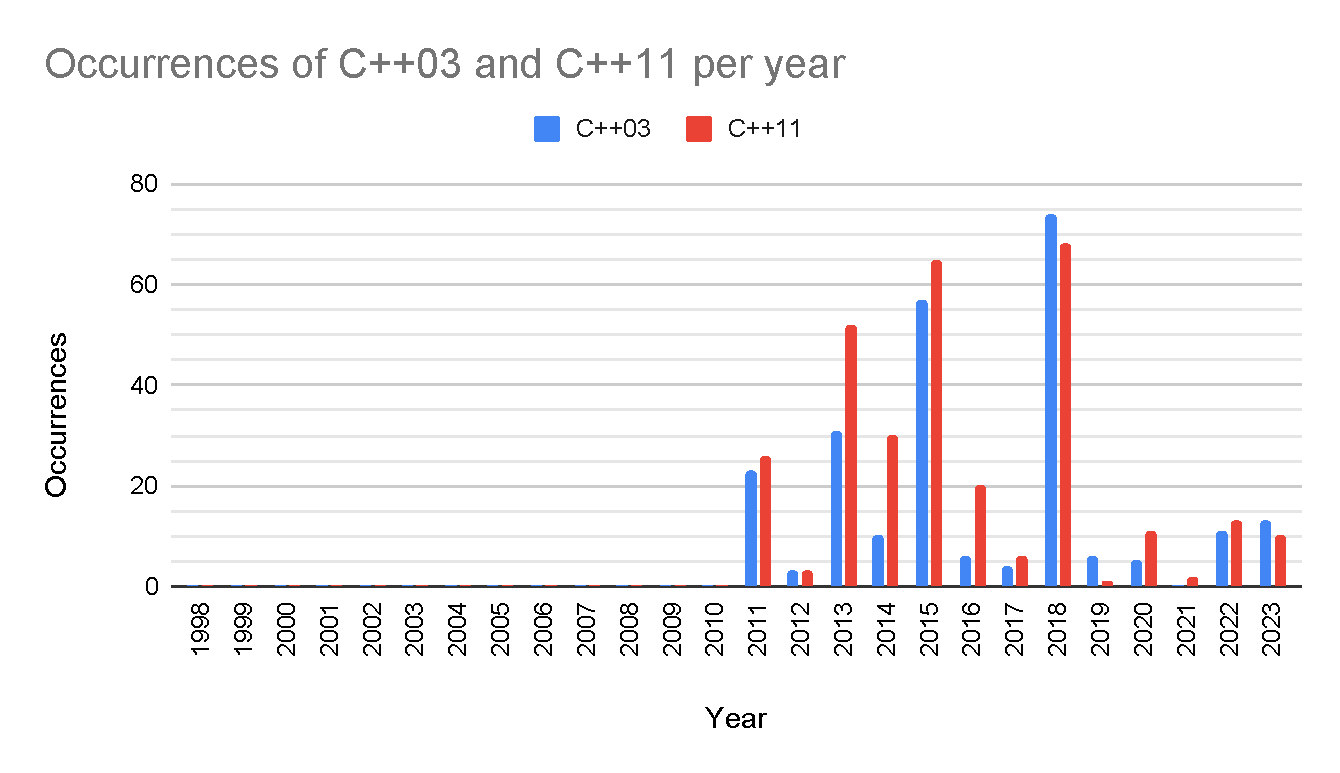
\includegraphics[width=\linewidth]{images/cpp03_11_year.pdf}
  \caption{Distribution of occurrences of C++03 (blue) and C++11 (red) by year}
  %\Description{Histogram of occurrences of topics C++03 and C++11 by year. Both distribution's shapes are fairly similar to one another.}
  \label{fig:cpp03_11_year}
\end{figure}

\begin{table*}
\caption{Mutual occurrences between code rejuvenation topics}
  \label{tab:mut_occurr}
\begin{tabular}{@{}lcccccccc@{}}
\toprule
                                    & \multicolumn{1}{l}{General} & \multicolumn{1}{l}{Compilers} & \multicolumn{1}{l}{C++98} & \multicolumn{1}{l}{\textbf{C++03}} & \multicolumn{1}{l}{\textbf{C++11}} & \multicolumn{1}{l}{C++14} & \multicolumn{1}{l}{C++17} & \multicolumn{1}{l}{C++20} \\ \midrule
\multicolumn{1}{l|}{General}        & -                           & 2                             & 0                         & 2                                  & 0                                  & 0                         & 0                         & 0                         \\
\multicolumn{1}{l|}{Compiler}      & 2                           & -                             & 6                         & 26                                 & 33                                 & 7                         & 8                         & 1                         \\
\multicolumn{1}{l|}{C++98}          & 0                           & 6                             & -                         & 14                                 & 18                                 & 8                         & 5                         & 0                         \\
\multicolumn{1}{l|}{\textbf{C++03}} & 2                           & 26                            & 14                        & -                                  & \textbf{188}                       & 29                        & 24                        & 10                        \\
\multicolumn{1}{l|}{\textbf{C++11}} & 0                           & 33                            & 18                        & \textbf{188}                       & -                                  & 72                        & 38                        & 10                        \\
\multicolumn{1}{l|}{C++14}          & 0                           & 7                             & 8                         & 29                                 & 72                                 & -                         & 27                        & 5                         \\
\multicolumn{1}{l|}{C++17}          & 0                           & 8                             & 5                         & 24                                 & 38                                 & 27                        & -                         & 10                        \\
\multicolumn{1}{l|}{C++20}          & 0                           & 1                             & 0                         & 10                                 & 10                                 & 5                         & 10                        & -                         \\ \bottomrule
\end{tabular}
\end{table*}


\begin{table*}
\caption{Percentage of mutual occurrences between code rejuvenation topics}
  \label{tab:mut_occurr_prop}
\begin{tabular}{@{}lcccccccc@{}}
\toprule
                                    & \multicolumn{1}{l}{General} & \multicolumn{1}{l}{Compilers} & \multicolumn{1}{l}{C++98} & \multicolumn{1}{l}{\textbf{C++03}} & \multicolumn{1}{l}{\textbf{C++11}} & \multicolumn{1}{l}{C++14} & \multicolumn{1}{l}{C++17} & \multicolumn{1}{l}{C++20} \\ \midrule
\multicolumn{1}{l|}{General}        & -                           & 1,5\%                         & 0,0\%                     & 1,5\%                              & 0,0\%                              & 0,0\%                     & 0,0\%                     & 0,0\%                     \\
\multicolumn{1}{l|}{Compiler}      & 1,7\%                       & -                             & 5,1\%                     & 22,0\%                             & 28,0\%                             & 5,9\%                     & 6,8\%                     & 0,8\%                     \\
\multicolumn{1}{l|}{C++98}          & 0,0\%                       & 23,1\%                        & -                         & 53,8\%                             & 69,2\%                             & 30,8\%                    & 19,2\%                    & 0,0\%                     \\
\multicolumn{1}{l|}{\textbf{C++03}} & 0,8\%                       & 10,7\%                        & 5,8\%                     & -                                  & \textbf{77,4\%}                    & 11,9\%                    & 9,9\%                     & 4,1\%                     \\
\multicolumn{1}{l|}{\textbf{C++11}} & 0,0\%                       & 10,7\%                        & 5,9\%                     & \textbf{61,2\%}                    & -                                  & 23,5\%                    & 12,4\%                    & 3,3\%                     \\
\multicolumn{1}{l|}{C++14}          & 0,0\%                       & 7,9\%                         & 9,0\%                     & 32,6\%                             & 80,9\%                             & -                         & 30,3\%                    & 5,6\%                     \\
\multicolumn{1}{l|}{C++17}          & 0,0\%                       & 12,1\%                        & 7,6\%                     & 36,4\%                             & 57,6\%                             & 40,9\%                    & -                         & 15,2\%                    \\
\multicolumn{1}{l|}{C++20}          & 0,0\%                       & 7,1\%                         & 0,0\%                     & 71,4\%                             & 71,4\%                             & 35,7\%                    & 71,4\%                    & -                         \\ \bottomrule
\end{tabular}
\end{table*}


\begin{table*}
\caption{Multiplied percentage of mutual occurrences between code rejuvenation topics}
  \label{tab:mut_occurr_mux}
\begin{tabular}{@{}lcccccccc@{}}
\toprule
                                    & \multicolumn{1}{l}{General} & \multicolumn{1}{l}{Compilers} & \multicolumn{1}{l}{C++98} & \multicolumn{1}{l}{\textbf{C++03}} & \multicolumn{1}{l}{\textbf{C++11}} & \multicolumn{1}{l}{C++14} & \multicolumn{1}{l}{C++17} & \multicolumn{1}{l}{C++20} \\ \midrule
\multicolumn{1}{l|}{General}        & -                           & 0,0\%                         & 0,0\%                     & 0,0\%                              & 0,0\%                              & 0,0\%                     & 0,0\%                     & 0,0\%                     \\
\multicolumn{1}{l|}{Compilers}      & 0,0\%                       & -                             & 1,2\%                     & 2,4\%                              & 3,0\%                              & 0,5\%                     & 0,8\%                     & 0,1\%                     \\
\multicolumn{1}{l|}{C++98}          & 0,0\%                       & 1,2\%                         & -                         & 3,1\%                              & 4,1\%                              & 2,8\%                     & 1,5\%                     & 0,0\%                     \\
\multicolumn{1}{l|}{\textbf{C++03}} & 0,0\%                       & 2,4\%                         & 3,1\%                     & -                                  & \textbf{47,4\%}                    & 3,9\%                     & 3,6\%                     & 2,9\%                     \\
\multicolumn{1}{l|}{\textbf{C++11}} & 0,0\%                       & 3,0\%                         & 4,1\%                     & \textbf{47,4\%}                    & -                                  & 19,0\%                    & 7,1\%                     & 2,3\%                     \\
\multicolumn{1}{l|}{C++14}          & 0,0\%                       & 0,5\%                         & 2,8\%                     & 3,9\%                              & 19,0\%                             & -                         & 12,4\%                    & 2,0\%                     \\
\multicolumn{1}{l|}{C++17}          & 0,0\%                       & 0,8\%                         & 1,5\%                     & 3,6\%                              & 7,1\%                              & 12,4\%                    & -                         & 10,8\%                    \\
\multicolumn{1}{l|}{C++20}          & 0,0\%                       & 0,1\%                         & 0,0\%                     & 2,9\%                              & 2,3\%                              & 2,0\%                     & 10,8\%                    & -                         \\ \bottomrule
\end{tabular}
\end{table*}

This could be an indicator for a deeper relation regarding both topics. To analyze this further, we computed all mutual occurrences between every pair of topics into Table \ref{tab:mut_occurr}. From this table it is possible to see that C++03 and C++11 occurred together a total of 188 times. This is also the largest amount of any other pair of topics in the table, the second largest being 72 occurrences between C++11 and C++14.

From Table \ref{tab:mut_occurr}, we computed what the amount of mutual occurrences represented from each topic's total occurrence number. The results of this are present in Table \ref{tab:mut_occurr_prop}. We see that the 188 mutual occurrences represented 77.4\% of C++03's total amount of occurrences. For C++11, it represented 61.2\%.

Table \ref{tab:mut_occurr_prop}, however, has many high-percentage cells, some even higher than the two mentioned. This can be due to two factors: One is that the topic in question was only mentioned when another topic also was, but not vice-versa. Another is that the topic in question simply has very low occurrence amount, therefore a high percentage represents only a few mutual occurrences. In both cases, the high percentage is not present on both sides of the occurrence relation. An example of this is the relation between C++20 and C++11: C++20 occurred 71.4\% alongside C++11, but we see that C++11 occurred only 3.3\% alongside C++20. Seeing as the total amount of mutual occurrences between these is only 10, this does not represent a tight relation between these two, rather, we argue it shows a dependance of one topic onto another, but not the other way around.

For that reason, we decided to multiply both percentage scores from each side of the mutual relations represented in Table \ref{tab:mut_occurr_prop}. By multiplying percentages, the result will only be a high number if both sides of the relation represent a high percentage, and will tend sharply to zero if one percentage is very low, prioritizing larger numbers better than taking the average of them. That result is what we see in Table \ref{tab:mut_occurr_mux}. The highest percentage score is seen between C++03 and C++11, and by a fairly large margin, being more than twice as much as the second highest percentage.

\textbf{These results confirm that C++03 and C++11 occurred together more often than not, being the most mutually occurring - both in total amount and in proportion - of every pair of topics.} This also shows that there were some minor mutual occurring relations between C++11 and C++14, C++14 and C++17, and finally C++17 and C++20.



\subsection{Arguments}

To answer research question (3), we started off by classifying every message with a rejuvenation bias of its own. This represents the overall meaning of the whole message, that may contain arguments of all different sorts and rejuvenation biases. \textbf{Of the 603 messages analyzed, we found that 354 (58.7\%) were in favor of rejuvenation efforts, while 140 (23.2\%) were against rejuvenation efforts and 109 (18.1\%) were ambiguous or neutral towards rejuvenation. This suggests an overall imbalance of presence in favor of rejuvenation in the discussions.} This does not answer the question fully, however, as it would be of interest to look at the arguments used in every message individually.

For that, we used the list of argument categories mentioned previously. This list contained 28 arguments that were separated in groups regarding their rejuvenation bias, as "in favor of rejuvenation", "against rejuvenation" and "ambiguous/neutral". From the manual analysis process we computed the number of occurrences for every argument, and from that how much they were present in the analyzed messages, which is what is presented in Table \ref{tab:argument_list}.

\begin{table*}
\caption{Argument list with rejuvenation bias, occurrence count and presence in analyzed messages}
  \label{tab:argument_list}
\begin{tabular}{@{}lccc@{}}
\multicolumn{1}{c}{\textbf{Argument}}          & \textbf{Rejuvenation Bias} & \textbf{Occurrence count} & \textbf{Presence} \\ \midrule
Against obstruction of new standards           & In favor                   & 35                        & 5,8\%             \\
Considers users of newer standards             & In favor                   & 15                        & 2,5\%             \\
Decentralization                               & In favor                   & 11                        & 1,8\%             \\
\textbf{Deprecation / Discontinuation}         & \textbf{In favor}          & \textbf{167}              & \textbf{27,7\%}   \\
Dissatisfaction with resistance to modernizing & In favor                   & 12                        & 2,0\%             \\
In favor of rejuvenation                       & In favor                   & 112                       & 18,6\%            \\
Invest in C++ innovation                       & In favor                   & 48                        & 8,0\%             \\
Maintenance cost of older standards            & In favor                   & 74                        & 12,3\%            \\
Modularization                                 & In favor                   & 44                        & 7,3\%             \\
Obsolescence argument                          & In favor                   & 19                        & 3,2\%             \\
Optimism with newer standards' adoption        & In favor                   & 18                        & 3,0\%             \\
Recommends updating standards                  & In favor                   & 20                        & 3,3\%             \\
Questions motivation for using older standards & In favor                   & 7                         & 1,2\%             \\
Against deprecation / discontinuation          & Against                    & 53                        & 8,8\%             \\
Against versioning                             & Against                    & 13                        & 2,2\%             \\
Considers users of older standards             & Against                    & 85                        & 14,1\%            \\
Cost of updating to newer standards            & Against                    & 29                        & 4,8\%             \\
In resistance to rejuvenation                  & Against                    & 38                        & 6,3\%             \\
Pessimism with newer standards' adoption       & Against                    & 24                        & 4,0\%             \\
Problem in newer standard                      & Against                    & 3                         & 0,5\%             \\
Unable to rejuvenate                           & Against                    & 9                         & 1,5\%             \\
Considers retrocompatibility                   & Ambiguous / Neutral        & 60                        & 10,0\%            \\
Descriptive                                    & Ambiguous / Neutral        & 70                        & 11,6\%            \\
Interdependence problems                       & Ambiguous / Neutral        & 73                        & 12,1\%            \\
Relevance argument                             & Ambiguous / Neutral        & 49                        & 8,1\%             \\
Questions motivation for using newer standards & Ambiguous / Neutral        & 6                         & 1,0\%             \\
Cynicism with community acceptance             & Ambiguous / Neutral        & 13                        & 2,2\%             \\
Versioning                                     & Ambiguous / Neutral        & 91                        & 15,1\%           
\end{tabular}
\end{table*}

We found that the ten most used argument categories were:

\begin{enumerate}
    \item Deprecation / Discontinuation (present in 27.7\% of messages)
    \item In favor of rejuvenation (18.6\%)
    \item Versioning (15.1\%)
    \item Considers users of older standards (14.1\%)
    \item Maintenance cost of older standards (12.3\%)
    \item Interdependence problems (12.1\%)
    \item Descriptive (11.6\%)
    \item Considers retrocompatibility (10.0\%)
    \item Against deprecation / discontinuation (8.8\%)
    \item Relevance argument (8.1\%)
\end{enumerate}

Of these, (1), (2) and (5) were in favor of rejuvenation, expressing, respectively, arguments towards discontinuation of support to older C++ standards, a general opinion in favor of a proposed rejuvenation effort, and citing the costs of continuing to support older standards. Arguments (3), (6) and (8) were considered ambiguous, expressing respectively that versioning could be applied to resolve a rejuvenation issue, saying there was a problem due to strong dependences over many libraries related to rejuvenation, and considered the effort should keep code compatible with older code. Arguments (7) and (10) were considered conceptually neutral, as they were the act of describing in detail a technical aspect to support your position on the matter, or arguing for the relevance or validity of a previous argument made. Finally, (4) and (9) were against rejuvenation, proposing respectively that developers should consider continuing support for users of older C++ standards, and that they were against discontinuation of these standards.

Not included in the list, but next in presence, were two more arguments in favor of rejuvenation that, along with argument (6), characterized the Boost environment and their unique ambitions and problems. These arguments are "(11) Invest in C++ innovation" (8.0\% presence), that expressed a desire to develop in very modern C++ standards in order to create new libraries and tools that could be incorporated into a future standard, and "(12) Modularization" (7.3\% presence) that expressed a desire to reduce the strong linkage between libraries at Boost in order to better resolve rejuvenation issues.

At Boost, some developers expressed concerns and ambitions regarding reestablishing the previous status of Boost as an organization that contributed majorly to C++'s standardization. That they were, regarding C++98 and C++03, but less so from C++11 onwards, which justified the call for considering this objective as a core priority in the group. Also closely related to Boost, their method of distribution and library usage is largely monolithic in nature, and very interconnected between a large number of libraries, which results in an extensive list of dependencies for a lot of Boost functionalities. This is prone to cause many problems in linkage, compilation and runtime, as different libraries are, at launch, free to be written in any modern C++ standard. Throughout the analyzed messages, we saw many messages around issues that regarded library X's developers proposing moving to a newer C++ standard, but being dissuaded from doing so due to library Y's developers, that closely depended on X, not approving of discontinuing support for older C++ standards.

Moreover, of these results and shown in Figure \ref{fig:arg_occurr}, we observe that 48.7\% of arguments used were in favor of rejuvenation, while ambiguous or neutral arguments represented 30.3\% of the total, and arguments against represented only 21.0\%. \textbf{This shows more than double the occurrence of arguments in favor of rejuvenation than there were of arguments against it.} However, since almost a third of arguments used were not clearly defined as to their rejuvenation bias, the overall distribution still remains unclear. For that, we analyzed this group of arguments in further depth.

\begin{figure}[h]
  \centering
  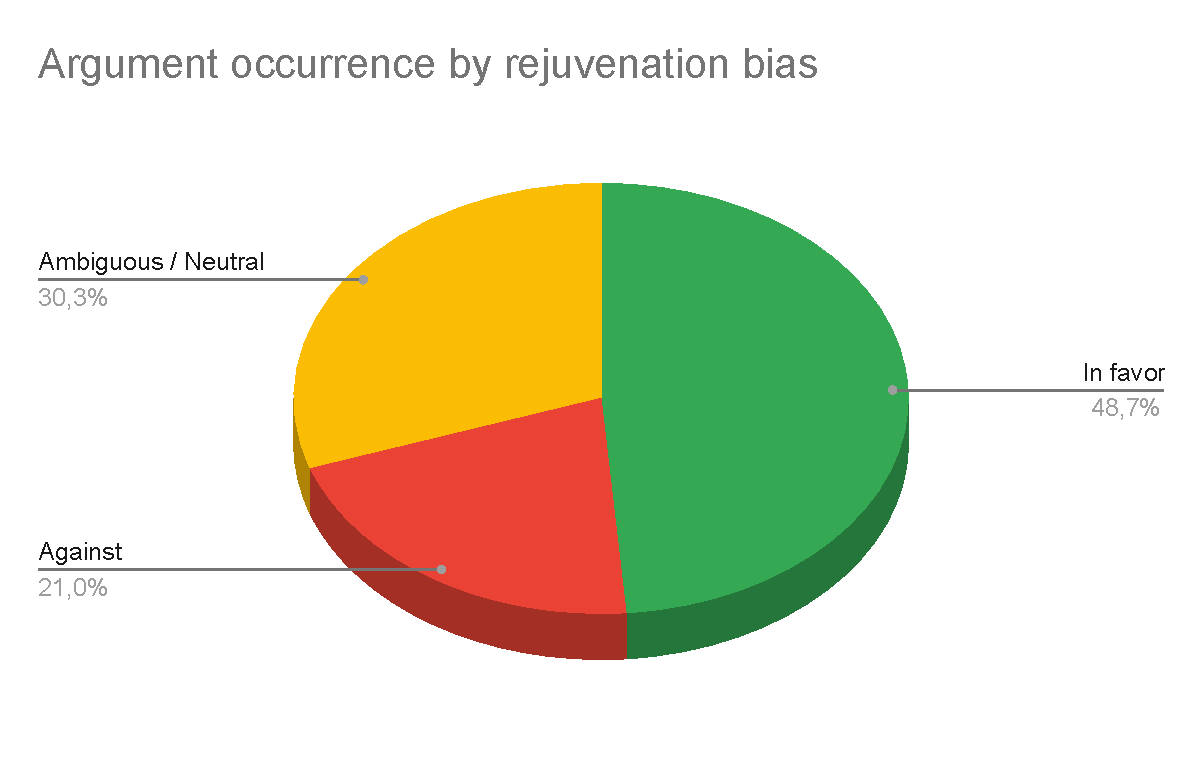
\includegraphics[width=\linewidth]{images/arg_occurr.pdf}
  \caption{Proportion of occurrences of arguments within rejuvenation discussion}
%  \Description{A pie graph showing the proportions of occurrences of each group of arguments regarding rejuvenation bias.}
  \label{fig:arg_occurr}
\end{figure}

Of this category of arguments, some were conceptually neutral, like "Descriptive" and "Relevance argument", due to their generalist nature of being discussion tools. That is, both of these express no opinion towards rejuvenation itself, they only explain a related topic in detail or question the relevance and validity of a previous argument in the discussion, and therefore can, in principle, be used equally in both sides of the discussion. However, other arguments in this category were not clearly defined as being predominantly in favor or against rejuvenation.

To determine whether an argument category previously classified as ambiguous had any bias towards rejuvenation, we looked at the classification of the messages where these arguments were found in. Figure \ref{fig:ambg_arg_occurr} shows the total number of occurrences of these arguments, along with sections of how many of these occurred in messages considered in favor of (green), against (red), ambiguous or neutral (yellow) to rejuvenation.

\begin{figure}[h]
  \centering
  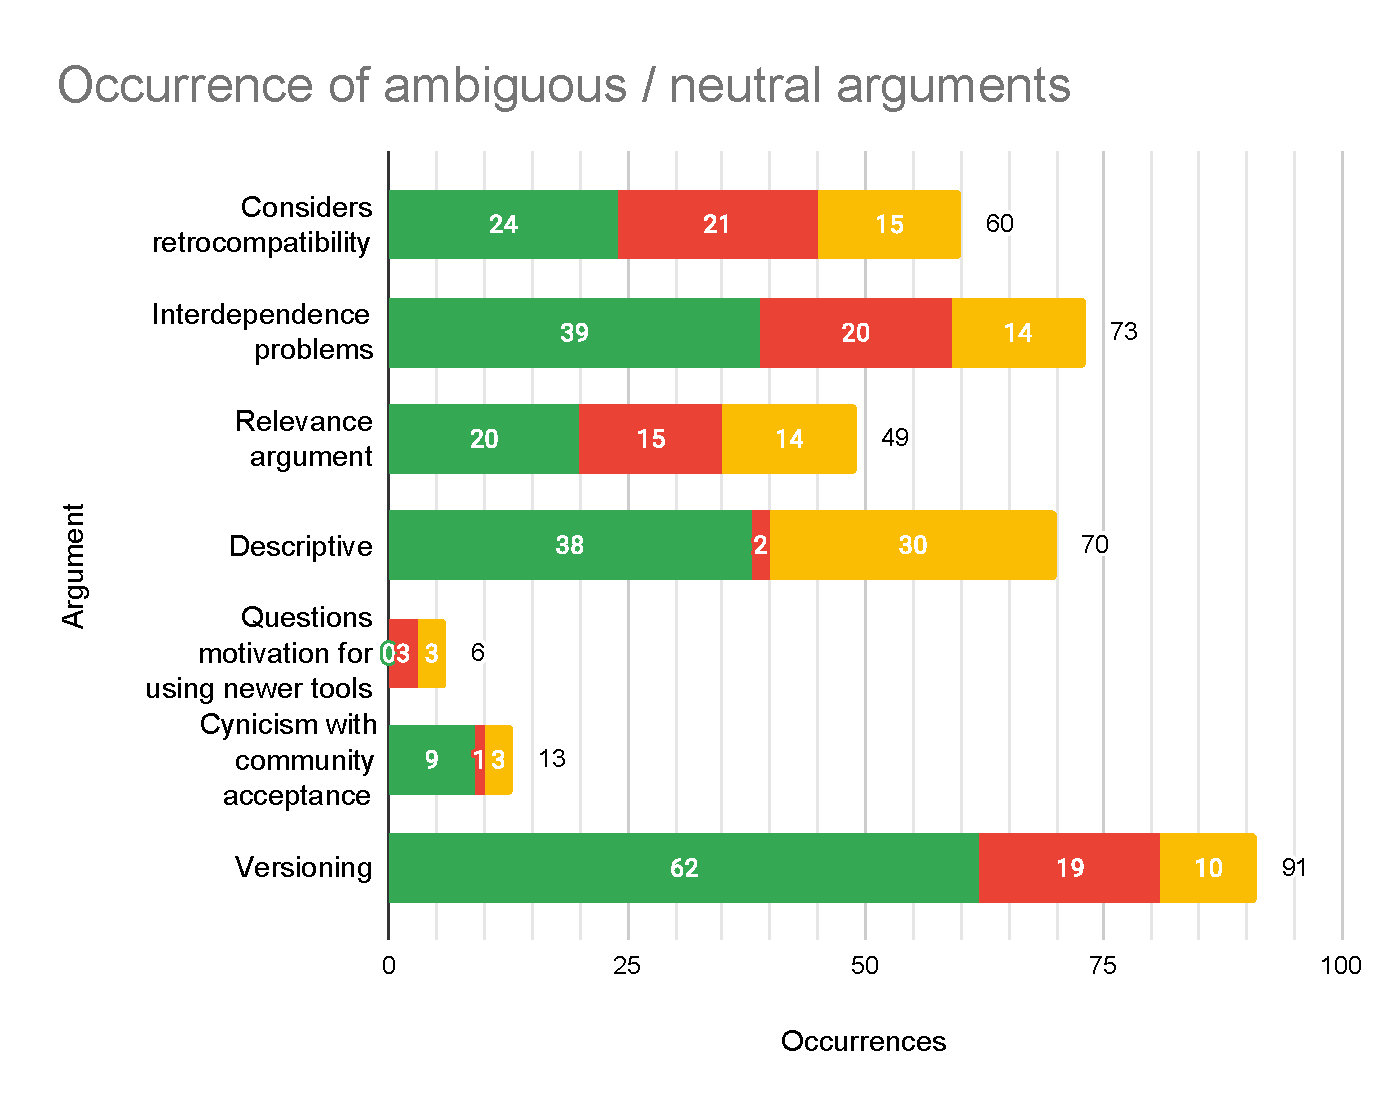
\includegraphics[width=\linewidth]{images/ambg_arg_occurr.pdf}
  \caption{Occurrences of ambiguous or neutral arguments separated by bias of the message they were utilized in}
%  \Description{A bar graph showing the occurrences of this category of arguments and the proportions of occurrences in messages of different rejuvenation biases.}
  \label{fig:ambg_arg_occurr}
\end{figure}

From this analysis, we found that arguments such as "Versioning", "Interdependence problems" and "Cynicism with community acceptance" were proportionally more employed in messages classified as in favor of rejuvenation, ranging from 53.4\% to 69.2\% of usage. In contrast, "Questioning motivation for using newer standards" seemed to be mostly used to argue against rejuvenation. Addittionally, "Considering retrocompatibility" was found to be used rather evenly by both sides, with the ambiguous use also being fairly present (25\% of occurrences). "Relevance argument" saw similar usage as the previous ambiguous argument. "Descriptive" was used often by messages in favor of rejuvenation (54.3\%), but almost just as often in ambiguous or neutral messages (42.9\%), which keeps it in an ambiguous or neutral classification.

\textbf{Overall, most uses of "Ambiguous / Neutral" arguments were in messages classified as in favor of rejuvenation. This solidifies the suggested positive bias towards rejuvenation in the arguments found in these discussions.}




\section{Threats to validity}
{\color{red} To do: Detail and explain the most relevant aspects to the study method that could pose as problematic to the validity of its results.}

\section{Conclusion}

In summary, these are the findings presented over this document.

\subsection{Prevalence}

\textbf{Research question (1): What is the prevalence of code rejuvenation discussions in the Boost mailing list?}

The overall presence of code rejuvenation discussion is likely less than 1\% of the total amount of messages in the Boost mailing list. These discussions became more prevalent after C++11's release, and saw a further increase in presence throughout reduced usage of the list in more recent years. Additionally, the discussions seemed to peak around new C++ standard releases.

\subsection{Topics}

\textbf{Research question (2): What were the most discussed topics? Which language standards were mentioned the most?}

The most discussed topics were C++11 and C++03, being present in around half of all 603 messages analyzed. These two topics were found to be mentioned together more often than not, and were tightly related in their occurrences. We also found that messages often mentioned more than one topic at once, and that they often discussed C++ standards that were 10+ years old, while more recent standards saw little presence in the discussion.

\subsection{Arguments}

\textbf{Research question: (3) What were the most common arguments in general? What were the most common ones either in favor of or against rejuvenation?}

The most used arguments in these discussions characterized conversations between developers proposing discontinuation of older C++ standards and citing the costs of maintaining these, while other developers argued against the proposal of discontinuation, majorly due to considering users of said older standards required this support. Often, keeping multiple versions in different C++ standards was proposed as a middle-ground compromise in favor of the rejuvenation proposal. In total amount, most arguments presented were in favor of rejuvenation.


\bibliographystyle{sbc}
\bibliography{sample-base}

\end{document}
